\section{Cơ sở lý thuyết về phần cứng và cảm biến}

Phần cứng của hệ thống đóng vai trò là nền tảng vật lý, nơi dữ liệu được thu thập và xử lý ban đầu. Việc lựa chọn các thiết bị phù hợp là rất quan trọng để đảm bảo tính hiệu quả và ổn định của toàn bộ hệ thống.

\subsection{Hệ thống nhúng và cảm biến}

Hệ thống nhúng là trái tim của thiết bị đeo trên người, đảm nhận vai trò thu thập và xử lý dữ liệu tại biên.

\subsubsection{Vi điều khiển (Microcontroller)}
Trong các dự án IoT hiện nay, có nhiều lựa chọn vi điều khiển rất phổ biến như Arduino, STM32 hay ESP32. Mỗi loại đều có những thế mạnh riêng, nhưng đối với đề tài này, \textbf{ESP32} được chọn vì những lý do rất thực tế. Vi điều khiển này không chỉ có khả năng xử lý mạnh mẽ với cấu trúc hai nhân, mà còn tích hợp sẵn Wi-Fi và Bluetooth. Điều này giúp thiết bị nhúng có thể dễ dàng kết nối với mạng và các thiết bị khác, đáp ứng đúng yêu cầu của hệ thống: vừa xử lý dữ liệu cảm biến, vừa liên lạc với máy chủ mà vẫn tiết kiệm năng lượng.
\begin{figure}[h]
    \centering
    
\includegraphics[width=0.8\textwidth]{esp32.jpg}
    \caption{Ví dụ về một module vi điều khiển ESP32.}
    \label{fig:esp32}
\end{figure}

\subsubsection{Cảm biến chuyển động quán tính (IMU)}
Đây là một trong những cảm biến quan trọng nhất để phát hiện té ngã. Một IMU tiêu biểu sẽ tích hợp hai loại cảm biến chính:
\begin{itemize}
    \item \textbf{Gia tốc kế:} Chịu trách nhiệm đo lường gia tốc của vật thể. Trong trường hợp té ngã, nó sẽ ghi nhận một cú va chạm mạnh và đột ngột.
    \item \textbf{Con quay hồi chuyển:} Giúp đo lường tốc độ góc, tức là sự thay đổi tư thế của người dùng. Dữ liệu từ con quay hồi chuyển rất hữu ích để nhận biết một người đang đứng thẳng chuyển sang nằm ngang.
\end{itemize}
Bằng cách kết hợp dữ liệu từ cả hai, hệ thống có thể phân biệt té ngã với các chuyển động đột ngột thông thường, từ đó tăng độ chính xác đáng kể.
\begin{figure}[h]
    \centering
    
\includegraphics[width=0.8\textwidth]{imu.png}
    \caption{Sơ đồ minh họa nguyên lý hoạt động của cảm biến IMU.}
    \label{fig:imu_working_principle}
\end{figure}

\subsubsection{Module định vị toàn cầu (GPS)}
Module GPS có nhiệm vụ xác định vị trí chính xác của thiết bị thông qua tín hiệu vệ tinh. Trong đề tài này, GPS đóng vai trò đặc biệt quan trọng khi người dùng ra khỏi khu vực giám sát của camera. Nhờ có GPS, hệ thống có thể cung cấp tọa độ vị trí cụ thể của người gặp nạn, giúp việc cứu hộ trở nên nhanh chóng và hiệu quả hơn.

\subsection{Hệ thống giám sát hình ảnh và máy chủ xử lý}

Đây là "đôi mắt" và "bộ não" của hệ thống, nơi dữ liệu được xử lý và phân tích chuyên sâu.

\subsubsection{Thiết bị camera nhúng}
Camera nhúng có nhiệm vụ ghi lại luồng video trong thời gian thực. Đối với đề tài này, một module camera tích hợp sẵn vào vi điều khiển như ESP32-CAM được sử dụng. Ưu điểm của nó là chi phí thấp, dễ dàng tích hợp và có thể truyền dữ liệu qua Wi-Fi một cách thuận tiện.
\begin{figure}[h]
    \centering
    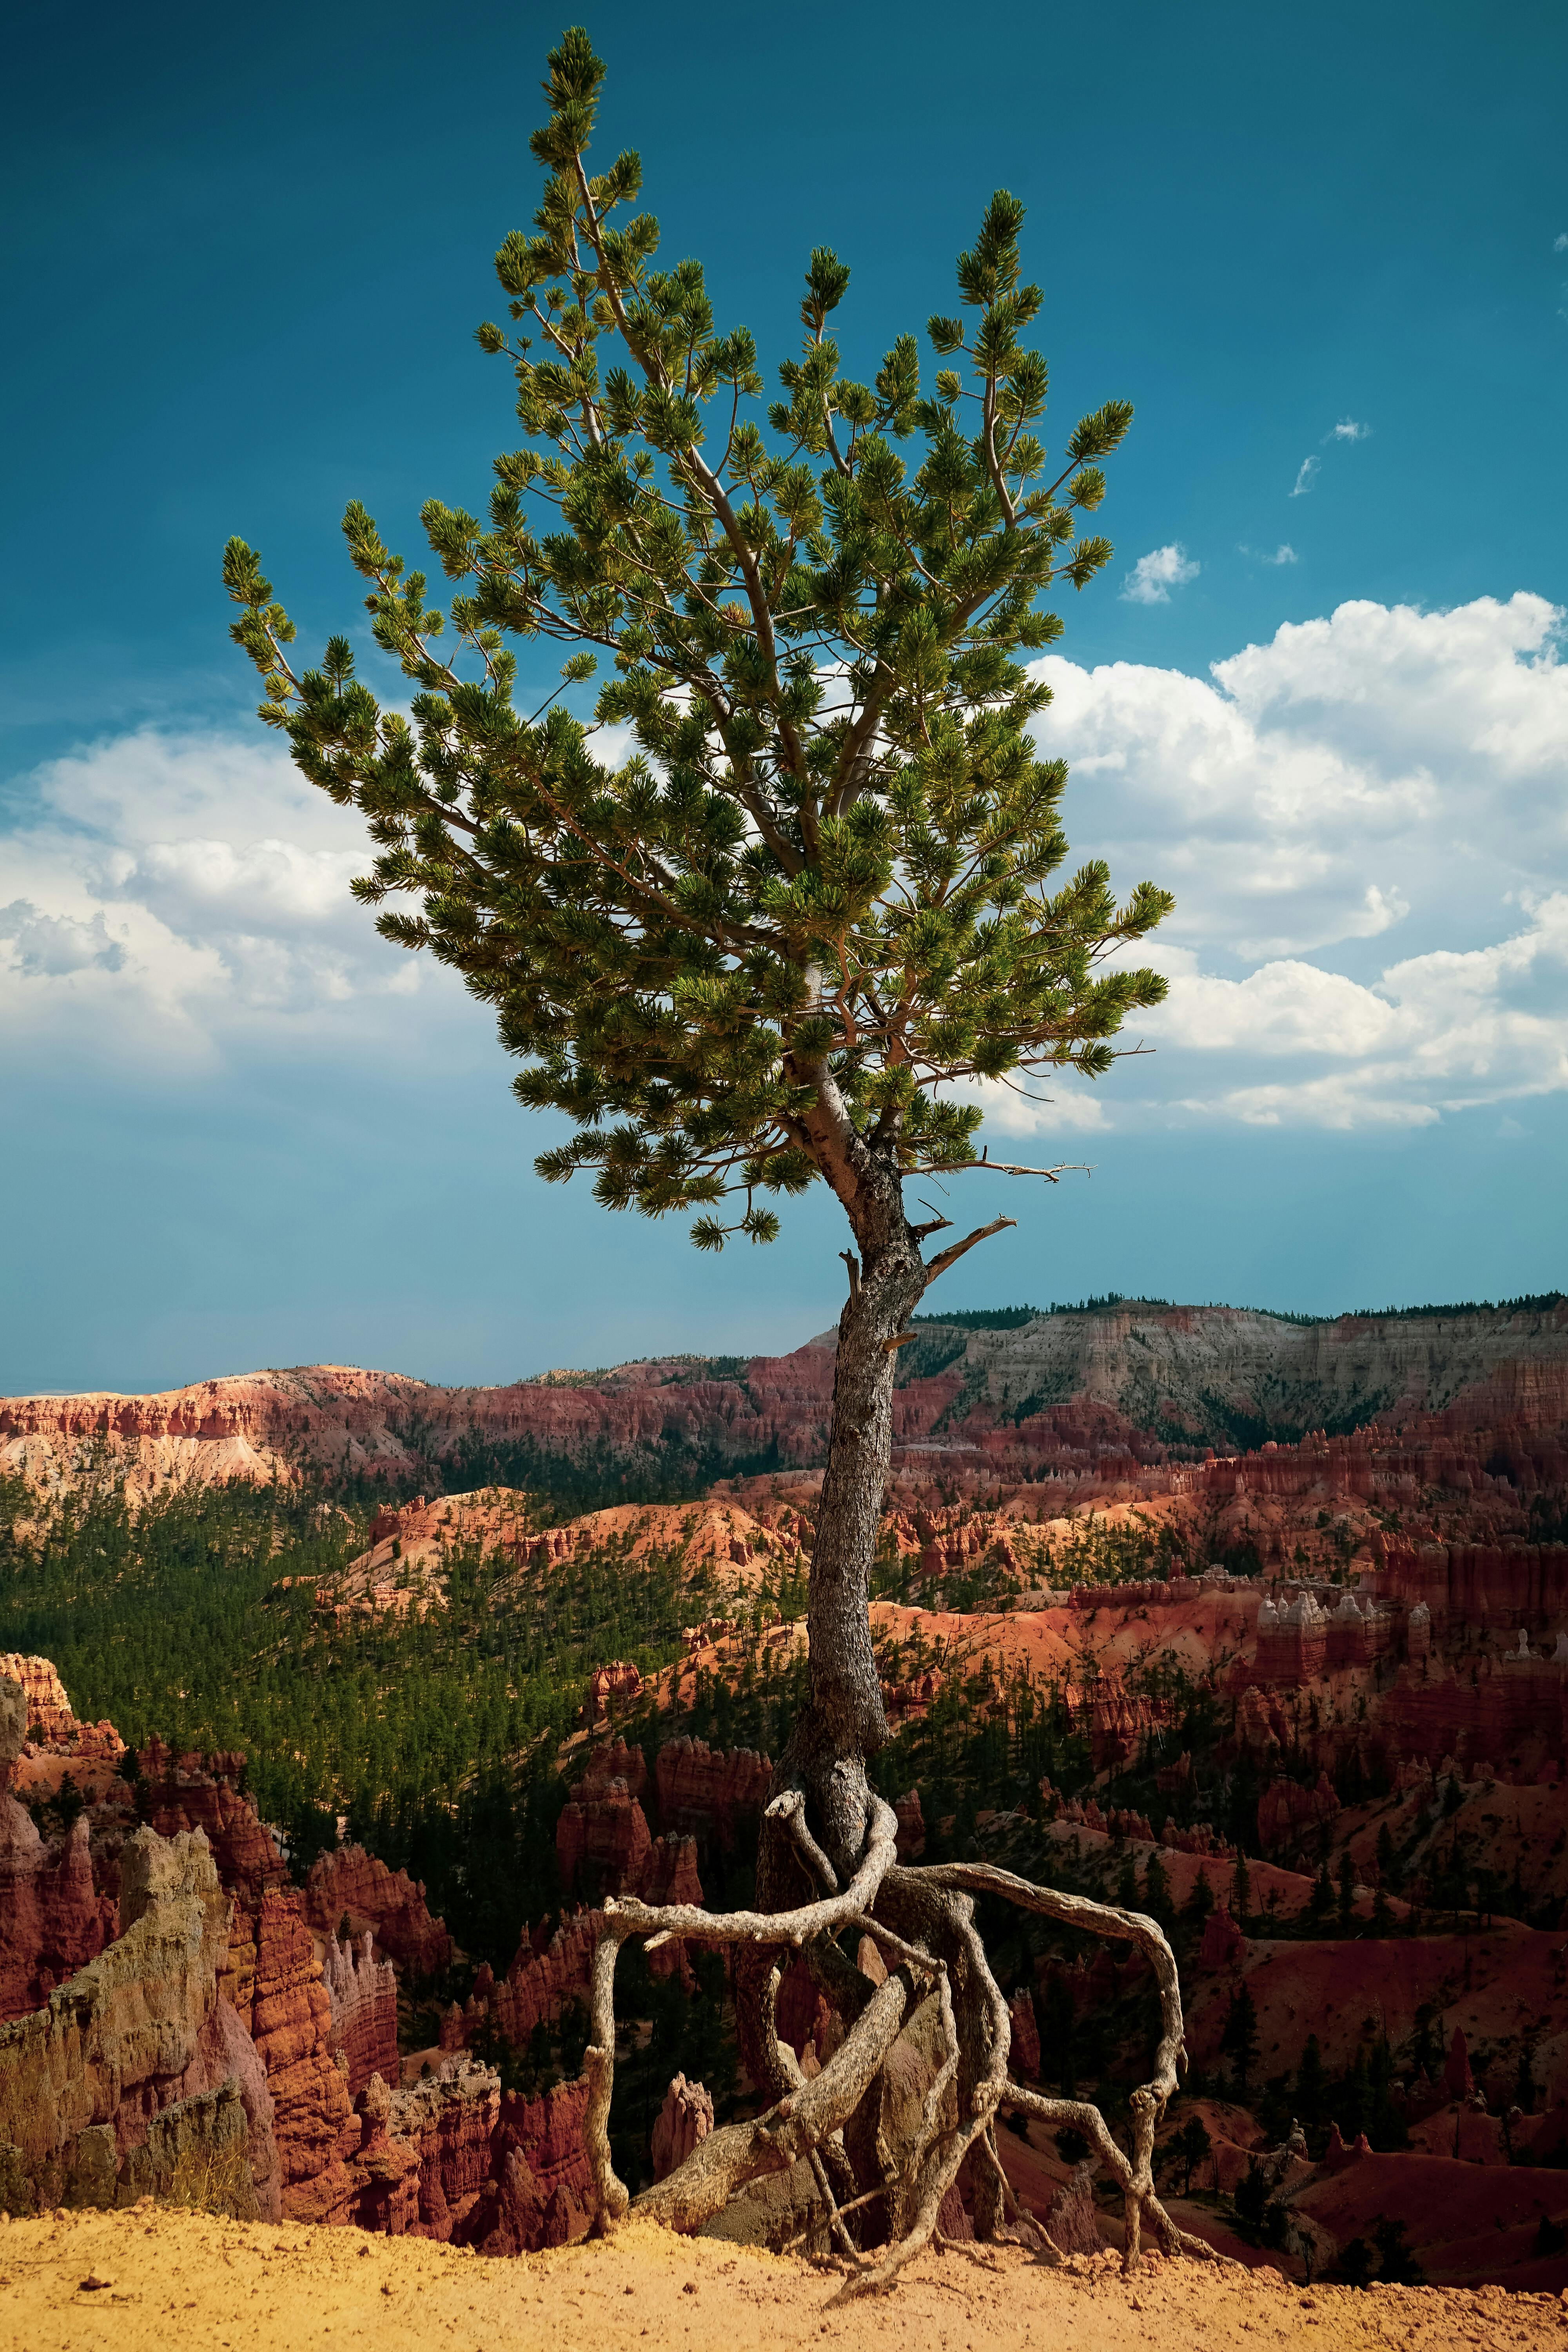
\includegraphics[width=0.8\textwidth]{camera_module.jpg}
    \caption{Một ví dụ về module camera nhúng tích hợp ESP32-CAM.}
    \label{fig:esp32_cam}
\end{figure}

\subsubsection{Máy chủ xử lý trung tâm}
Thay vì xử lý tất cả trên thiết bị nhúng, hệ thống tận dụng một máy chủ mạnh mẽ để làm công việc này. Máy chủ này chạy trên nền tảng Linux và sử dụng \textbf{Python} cùng với một hệ sinh thái thư viện khổng lồ như OpenCV và các công cụ học máy. Việc này giúp hệ thống có thể chạy các thuật toán phân tích hình ảnh phức tạp một cách hiệu quả, trong khi thiết bị nhúng tập trung vào việc thu thập dữ liệu và liên lạc.

\subsection{Hệ thống truyền thông di động và cố định}

Hệ thống truyền thông đóng vai trò đảm bảo các cảnh báo được gửi đi nhanh chóng và đáng tin cậy.

\subsubsection{Module truyền thông di động (4G/LTE)}
Module 4G cung cấp kết nối internet thông qua mạng di động, cho phép thiết bị hoạt động ở bất cứ đâu có sóng. Đây là chìa khóa để hệ thống có thể giám sát liên tục, ngay cả khi người dùng không ở trong tầm phủ Wi-Fi.

\subsubsection{Nền tảng máy chủ truyền thông}
Máy chủ trung tâm còn đóng vai trò là "trung tâm điều hành" các kênh truyền thông:
\begin{itemize}
    \item \textbf{Tổng đài SIP (Asterisk):} Giúp tạo ra một hệ thống gọi điện nội bộ qua mạng LAN, đảm bảo kênh cảnh báo dự phòng hoạt động độc lập với internet.
    \item \textbf{Giao thức MQTT:} Hỗ trợ việc gửi và nhận dữ liệu cảnh báo từ các thiết bị nhúng đến các ứng dụng giám sát từ xa một cách hiệu quả.
\end{itemize}
Sự kết hợp này tạo nên một hệ thống cảnh báo mạnh mẽ, có tính dự phòng và rất ổn định.
